\RequirePackage{fix-cm}
\documentclass[rgb,cdgeometry=no,cd=true,cdhead=bicolor,cdfont=false,cdfoot=color,cdfont=nodin,english,paper=A0,fontsize=32pt,DIV=25,usegeometry]{tudscrposter}
\usepackage[rgb]{xcolor}
\usepackage{selinput}\SelectInputMappings{adieresis={ä},germandbls={ß}}
\usepackage[T1]{fontenc}
\usepackage{microtype}
\usepackage{csquotes}
\usepackage{enumitem}

\usepackage{tikz}
\usetikzlibrary{shapes.arrows,calc}

\usepackage{ifthen}
\usepackage{environ}
\usepackage[english]{babel}
\usepackage[hidelinks]{hyperref}
\usepackage{geometry}
\usepackage[absolute]{textpos}

\usepackage{tudscrcolor}
% some colors are currently missing in tudscrcolor
\definecolor{tudcyan}{cmyk/RGB/rgb}{%
	1.00,0.00,0.00,0.00/000,158,224/0.0,0.6196078431372549,0.8784313725490196%
}%

\definecolor{boxbg}{RGB}{205,212,226}
\definecolor{boxfg}{RGB}{0,29,75}


\definecolor{tudgrey}{RGB}{95,99,98}

\newcommand{\vboxsep}{\par\vspace{16mm}\noindent\hspace*{-2mm}}
\newcommand{\clinesep}{\par\vspace{12mm}\noindent\hspace*{-2mm}}
\newcommand{\hboxsep}{\hspace{11mm}}

\DeclareRobustCommand\ebseries{\fontseries{eb}\selectfont}
\DeclareRobustCommand\nbseries{\fontseries{b}\selectfont}
\DeclareRobustCommand\sbseries{\fontseries{sb}\selectfont}
\DeclareRobustCommand\rgseries{\fontseries{m}\selectfont}
\DeclareRobustCommand\ltseries{\fontseries{l}\selectfont}
\DeclareRobustCommand\clseries{\fontseries{cl}\selectfont}
\DeclareTextFontCommand{\texteb}{\ebseries}
\DeclareTextFontCommand{\textsb}{\sbseries}
\DeclareTextFontCommand{\textlt}{\ltseries}
\DeclareTextFontCommand{\textcl}{\clseries}


\newcommand{\boxheadline}[1]{\textbf{\fontsize{36pt}{500pt}\selectfont{#1}}\par\vspace{3mm}}

\newcommand{\titlebox}[2]{
    \begin{tikzpicture}[remember picture,overlay]
    \node at (current page.north west) {
        \begin{tikzpicture}[remember picture,overlay]
        \node[anchor=north west,align=left] at (28mm,-158mm) {
            \begin{minipage}{\linewidth}
            \setlength{\baselineskip}{85pt}
%            \textbf{\fontsize{40pt}{500pt}\selectfont{\textcolor{HKS41}{Software Language Engineering 2018}}}\par
            \textbf{\fontsize{80pt}{500pt}\selectfont{\textcolor{HKS41}{#1}}}\par
            \vspace{8mm}
            \setlength{\baselineskip}{44pt}
            \textsb{\fontsize{40pt}{500pt}\selectfont{\textcolor{HKS41}{#2}}}
            \end{minipage}
            
        };
        \end{tikzpicture}
    };
\end{tikzpicture}
}

\newcommand{\fgcolor}[2]{
%	\ifthenelse{\equal{#1}{TB1}}{\textcolor{TB1fg}{#2}}{
%		\ifthenelse{\equal{#1}{TB2}}{\textcolor{TB2fg}{#2}}{
%			\ifthenelse{\equal{#1}{TB3}}{\textcolor{TB3fg}{#2}}{
%				\textcolor{boxfg}{#2}	
%			}
%		}
%	}
  \textcolor{#1}{#2}
}
\newcommand{\bgcolorline}[2]{
	\ifthenelse{\equal{#1}{tudcyan}}{
		\node[anchor=north west,minimum height=25mm,fill=tudcyan!20,minimum width=#2,align=center,inner sep=0,line width=1mm,draw=tudcyan!20,outer sep=0] {};
		}{
	\ifthenelse{\equal{#1}{HKS41}}{
		\node[anchor=north west,minimum height=25mm,fill=HKS41!20,minimum width=#2,align=center,inner sep=0,line width=1mm,draw=HKS41!20,outer sep=0] {};
		}{
	\ifthenelse{\equal{#1}{HKS44}}{
		\node[anchor=north west,minimum height=25mm,fill=HKS44!20,minimum width=#2,align=center,inner sep=0,line width=1mm,draw=HKS44!20,outer sep=0] {};
		}{
	\ifthenelse{\equal{#1}{HKS07}}{
		\node[anchor=north west,minimum height=25mm,fill=HKS07!20,minimum width=#2,align=center,inner sep=0,line width=1mm,draw=HKS07!20,outer sep=0] {};
		}{
	\ifthenelse{\equal{#1}{HKS65}}{
		\node[anchor=north west,minimum height=25mm,fill=HKS65!20,minimum width=#2,align=center,inner sep=0,line width=1mm,draw=HKS65!20,outer sep=0] {};
	}{
		\node[anchor=north west,minimum height=25mm,fill=#1,minimum width=#2,align=center,inner sep=0,line width=1mm,draw=#1,outer sep=0] {};
  }
	}
	}
	}
	}
}

\newcommand{\bgcolorbox}[4]{
	\ifthenelse{\equal{#1}{HKS41}}{
		\node[anchor=north west,align=left,line width=1mm,draw=HKS41!20,outer sep=0] at (0,\dimexpr-25mm\relax) {
			\begin{minipage}[t][#3]{\dimexpr#2-8.3mm\relax}
				\vspace{3mm}
				#4
			\end{minipage}
		};
	}{
	\ifthenelse{\equal{#1}{tudcyan}}{
		\node[anchor=north west,align=left,line width=1mm,draw=tudcyan!20,outer sep=0] at (0,\dimexpr-25mm\relax) {
			\begin{minipage}[t][#3]{\dimexpr#2-8.3mm\relax}
				\vspace{3mm}
				#4
			\end{minipage}
		};
	}{
	\ifthenelse{\equal{#1}{HKS44}}{
		\node[anchor=north west,align=left,line width=1mm,draw=HKS44!20,outer sep=0] at (0,\dimexpr-25mm\relax) {
			\begin{minipage}[t][#3]{\dimexpr#2-8.3mm\relax}
				\vspace{3mm}
				#4
			\end{minipage}
		};
	}{
	\ifthenelse{\equal{#1}{HKS07}}{
  	\node[anchor=north west,align=left,line width=1mm,draw=HKS07!20,outer sep=0] at (0,\dimexpr-25mm\relax) {
  		\begin{minipage}[t][#3]{\dimexpr#2-8.3mm\relax}
  			\vspace{3mm}
  			#4
  		\end{minipage}
  	};
	}{
	\ifthenelse{\equal{#1}{HKS65}}{
  	\node[anchor=north west,align=left,line width=1mm,draw=HKS65!20,outer sep=0] at (0,\dimexpr-25mm\relax) {
  		\begin{minipage}[t][#3]{\dimexpr#2-8.3mm\relax}
  			\vspace{3mm}
  			#4
  		\end{minipage}
  	};
	}{
  	\node[anchor=north west,align=left,line width=1mm,draw=#1,outer sep=0] at (0,\dimexpr-25mm\relax) {
  		\begin{minipage}[t][#3]{\dimexpr#2-8.3mm\relax}
  			\vspace{3mm}
  			#4
  		\end{minipage}
  	};
	}
	}
	}
	}
	}
}

\NewEnviron{contentbox}[4][]{
	\begin{tikzpicture}
		\bgcolorline{#4}{#3}
		\node[anchor=north west,minimum height=25mm,,minimum width=#3,align=center,inner sep=7mm] {
			\fgcolor{#4}{\fontsize{45pt}{500pt}\selectfont{\textbf{#2}}}
		};
		\bgcolorbox{#4}{#3}{#1}{\BODY}
		\end{tikzpicture}
}

\NewEnviron{slimbox}[4][]{
	\begin{tikzpicture}
	\bgcolorline{#4}{#3}
	\node[anchor=north west,minimum height=25mm,,minimum width=#3,align=center,inner sep=7mm] {
		\fgcolor{#4}{\fontsize{45pt}{500pt}\selectfont{\textbf{#2}}}
	};
		\node[anchor=north west,align=left] at (0,\dimexpr-25mm\relax) {
	\begin{minipage}[t][#1]{\dimexpr#3-10.7mm\relax}
	\vspace{3mm}
	\BODY
	\end{minipage}
};
	\end{tikzpicture}
}

\newcommand{\floatline}[3]{
	\begin{tikzpicture}
	\bgcolorline{#3}{#2}
	\node[anchor=north west,minimum height=25mm,,minimum width=#2,align=center,inner sep=7mm,outer sep=0] {
		\fgcolor{#3}{\fontsize{45pt}{500pt}\selectfont{\textbf{#1}}}
	};
	\end{tikzpicture}
}

\let\OLDthebibliography\thebibliography
\renewcommand\thebibliography[1]{
  \OLDthebibliography{#1}
  \setlength{\parskip}{0pt}
  \setlength{\itemsep}{0pt plus 1ex}
}

\NewEnviron{literaturebox}{
    \begin{tikzpicture}[remember picture,overlay]
    \node at (current page.north west) {
        \begin{tikzpicture}[remember picture,overlay]
        \node[anchor=south west,align=left,inner sep=0,outer sep=0] at (32mm,-1069mm) {
            \begin{minipage}{\dimexpr777mm\relax}
            \setlength{\baselineskip}{32pt}
            \textcolor{tudgrey}{\fontsize{24pt}{5pt}\selectfont{\BODY}}
            \end{minipage}
        };
        \end{tikzpicture}
    };
\end{tikzpicture}
}

\usepackage{listings}
\usepackage{inconsolata}

\lstdefinestyle{common-style}{
  basicstyle=\scriptsize\ttfamily,  % the size of the fonts that are used for the code
  showspaces=false,                   % show spaces adding particular underscores
  showstringspaces=false,             % underline spaces within strings
  showtabs=false,                     % show tabs within strings adding particular underscores
%  frame=tlrb,                         % adds a frame around the code
  framexleftmargin=1em,               % space between left part of frame and listing
  tabsize=2,                          % sets default tabsize to 2 spaces
  breaklines=true,                    % sets automatic line breaking
  breakatwhitespace=true,             % sets if automatic breaks should only happen at whitespace
  keywordstyle={\color{blue}\textbf}, % keywords are blue
  commentstyle={\color{gray}},        % comments
  literate={\$}{{{\$}}}1,
  basewidth=0.5em,
  breakindent=40pt,
  breakautoindent=true,
  escapechar=\&,
  aboveskip={0.1\baselineskip}
}

\lstdefinestyle{shortlisting}{
	xleftmargin=\parindent,
	frame=none,
	aboveskip=3pt,belowskip=3pt
}

\lstdefinestyle{unboxed}{
  style=common-style,
	frame=none,
}

% JastAdd
\lstdefinelanguage{AST}{
	style=common-style,
	morekeywords={abstract,rel},
	otherkeywords={::=,->,<,>},
	morecomment=[l]{//}, morecomment=[s]{/*}{*/},
}

\lstdefinelanguage{JRAG}[]{java}{
	style=common-style,
	morekeywords={abstract,public,private,boolean,aspect,null,syn,inh,coll,eq,with,int,contributes,new,return,for,if,else,this,to,true,false},
	morecomment=[l]{//}, morecomment=[s]{/*}{*/},
}

\newcommand{\lstbg}[3][0pt]{{\fboxsep#1\colorbox{#2}{\strut #3}}}
\lstdefinelanguage{diff}[]{java}{
  style=common-style,
  morecomment=[f][\lstbg{HKS07!30}]-,
  morecomment=[f][\lstbg{HKS65!30}]+,
  morecomment=[f][\textit]{@@},
  %morecomment=[f][\textit]{---},
  %morecomment=[f][\textit]{+++},
}

\lstdefinestyle{AST} { language=AST,style=common-style } 
\lstdefinestyle{JRAG} { language=JRAG,style=common-style }
\lstdefinestyle{Java} { language=Java,style=common-style }


\usepackage{multirow}
\usepackage{booktabs}
\usepackage{amssymb}
\usepackage[default, scale=0.8]{opensans}

\usepackage{fontawesome5}
\newcommand{\thumbsup}{\faIcon[regular]{thumbs-up}}

%\renewcommand{\thebibliography}{}

\begin{document}
\setlength\oddsidemargin{6.7mm}%
\setlength\textwidth{777mm}%
\setlength\textheight{800mm}%
\setlength\footheight{31.3mm}%
\setlength{\topskip}{8mm}%
\setlength{\headsep}{110mm}%
\faculty[]{\hspace{-78mm} Software Language Engineering 2018}%
%\institute[]{Software Language Engineering 2018}%
\headlogo{images/lund-logo-neg.pdf}%
\noindent\hspace*{-4mm}%
\begin{tikzpicture}[remember picture,overlay]%
\node at (700mm,200mm) {
\includegraphics[width=50mm,page=1]{images/badges.pdf}};%
\node at (755mm,200mm) {
\includegraphics[width=50mm,page=2]{images/badges.pdf}};%
\end{tikzpicture}%
\begin{contentbox}[140mm]{Problem: Efficient Navigation of Non-containment References}{776mm}{HKS41}
\begin{minipage}{255mm}
%% Ecore model
Metamodel of the Trainbenchmark~\cite{szarnyas_train_2017}:\\
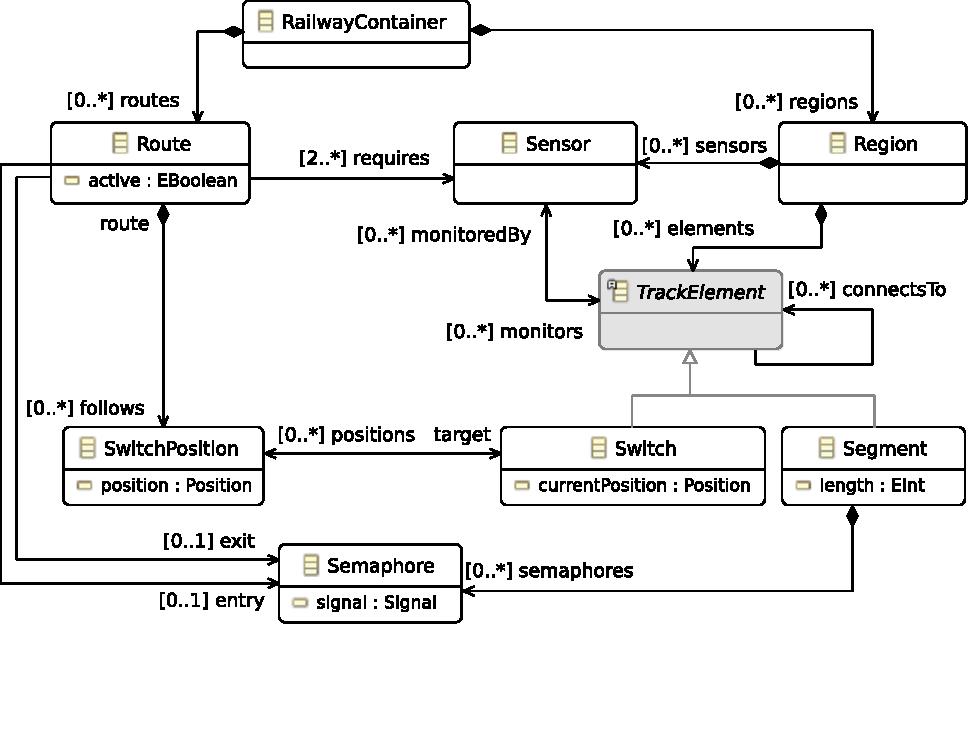
\includegraphics[height=150mm,keepaspectratio]{images/ecore-no-enums}
\end{minipage}
%% Arrows ecore -> runtime model
\begin{tikzpicture}[remember picture,overlay,
        fat arrow/.style={single arrow,thick,draw=HKS41!30,
                          single arrow head extend=40mm,
                          single arrow tip angle=130,
                          single arrow head extend=1mm,
                          fill=HKS41!10,minimum height=35mm,
                          minimum width=100mm}
]
\node at (-35mm,17mm) [fat arrow] {};
\end{tikzpicture}%
\begin{minipage}{140mm}
\vspace{-22mm}
%% Runtime model
\centering General Runtime model:\\
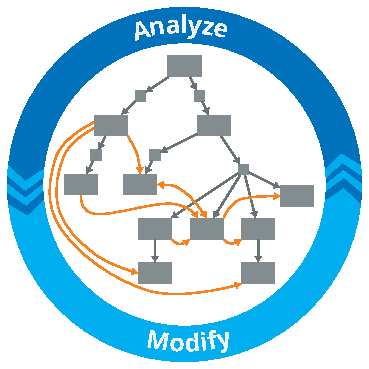
\includegraphics[height=130mm,keepaspectratio]{images/process-ag.pdf}
\end{minipage}
%% Zoom effect
\begin{tikzpicture}[remember picture,overlay]
\draw [draw=HKS33,line width=1mm] (-60mm,-12mm) rectangle (-50mm,-6mm);
\draw [draw=HKS33,thick,dashed] (-60mm,-6mm) -- (10mm,80mm); % left upper
%\draw [draw=HKS33,thick,dashed] (-50mm,-6mm) -- (10mm,40mm); % right upper
%\draw [draw=HKS33,thick,dashed] (-50mm,-12mm) -- (10mm,-30mm); % right lower
\draw [draw=HKS33,thick,dashed] (-60mm,-12mm) -- (10mm,-50mm); % left lower
% fill area with transparent color
\draw [fill=HKS33, opacity=0.2] (-60mm,-6mm) -- (10mm,80mm) -- (10mm,-50mm) -- (-60mm,-12mm) -- (-50mm,-12mm) -- (-50mm,-6mm);
% draw an rectangle around next minipage
\draw [draw=HKS33] (10mm,80mm) rectangle (350mm,-50mm);
\end{tikzpicture}%
\begin{minipage}{340mm}
\vspace{-22mm}
\begin{itemize}
\item RAGs~\cite{hedin2000reference} can be used for models@runtime providing some advantages
\begin{itemize}
\item \textit{Separation of structure and computation}
\item \emph{Shorthands} for navigation and computation on trees
\item \emph{Efficiency} through memoization of computed values
\item \textit{Incremental computation}, i.e., invalidating of outdated cached values
\end{itemize}
\item \textbf{Major issue:} Non-containment references can not be encoded \emph{efficiently} w.r.t. performance and consistency
\end{itemize}
\end{minipage}
\end{contentbox}
%% Arrows between variants
\begin{tikzpicture}[remember picture,overlay,
        fat arrow/.style={single arrow,thick,draw=HKS41!20,
                          single arrow head extend=30mm,
                          single arrow tip angle=160,
                          single arrow head extend=1mm,
                          fill=HKS41!8,minimum height=20mm,
                          minimum width=100mm}]
\node at (330mm,-180mm) [fat arrow] {};
\node at (512mm,-180mm) [fat arrow] {};
\end{tikzpicture}%
\vboxsep%
\vspace{5mm} % To adjust space between second and third part :)
%% Minipage for state-of-the-art boxes
\begin{minipage}{509mm}
%\vspace{-26mm}
\begin{contentbox}[60mm]{State-of-the-Art Using RAGs and JastAdd~\cite{jastadd}}{509mm}{HKS41}
%\centering
\begin{minipage}{285mm}
%% Shared grammar parts
%\boxheadline{Excerpt of the used grammar}
%Excerpt of the used grammar
\lstinputlisting[language=AST,style=unboxed]{code/refs-full.ast}
\end{minipage}
%
\begin{minipage}{220mm}
%% Shared attribute Route.requires()
%Example of an attribute for an inverse relation
\lstinputlisting[language=JRAG,style=unboxed,frame=l]{code/requiresNamelookup.jrag}
\end{minipage}
\end{contentbox}
\clinesep%
%% Namelookup box
\begin{contentbox}[106mm]{\quad Name Lookup}{326mm}{HKS07}
\begin{minipage}{135mm}
  \lstinputlisting[language=AST,style=unboxed]{code/refNamelookup.ast}
  \boxheadline{Idiomatic Approach}
  \lstinputlisting[language=JRAG,style=unboxed]{code/resolveNamelookup-Naive.jrag}
\end{minipage}
\begin{minipage}{196mm}
\begin{tikzpicture}[remember picture,overlay]
\draw (-5mm,10mm) -- (-5mm,-80mm);
\end{tikzpicture}
  \boxheadline{Idiomatic Approach with a Map}
  \lstinputlisting[language=JRAG,style=unboxed,basicstyle=\tiny\ttfamily]{code/resolveNamelookup-Tight.jrag}
\end{minipage}
\end{contentbox}
%
\hboxsep %
%% Intrinsic references box
\begin{contentbox}[106mm]{\quad Intrinsic References}{168mm}{tudcyan}
\lstinputlisting[language=AST,style=unboxed]{code/refOptimized.ast}
{
  \setlist{leftmargin=8mm}
  \begin{itemize}
    \item Name-Analysis done in deserializer and after every edit
    \item Faster evaluation and less cache invalidation
  \end{itemize}
}
\end{contentbox}
\end{minipage}
%
\hboxsep
%% Grammar extension box
\begin{minipage}{254mm}
%\vspace{-24mm}
\begin{contentbox}[210mm]{\quad Grammar Extension}{254mm}{HKS65}
\boxheadline{Introducing Relations}
\lstinputlisting[language=AST,frame=]{code/refSpecialized.ast}
\boxheadline{Adding the Preprocessor \emph{RelAst}}
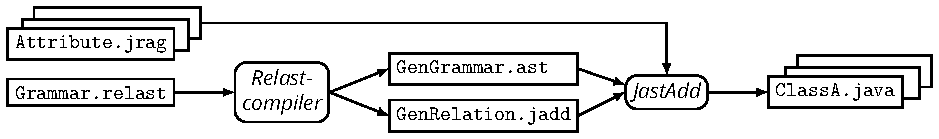
\includegraphics[width=240mm,keepaspectratio]{images/relast-process}
\boxheadline{Generated API}
\lstinputlisting[language=JRAG,style=unboxed]{code/requiresSpecialized.jrag}
\end{contentbox}
\end{minipage}
%% Draw the symbols for the legend onto the three content boxes, remember to create no newlines
\begin{tikzpicture}[remember picture, overlay]%
%% Coordinates
\coordinate (nl-no) at (105mm,134mm);
\coordinate (nl-inc) at (105mm,124mm);
\coordinate (opt-no) at (350mm,135mm);
\coordinate (opt-inc) at (350mm,125mm);
\coordinate (spec-no) at (570mm,238mm);
\coordinate (spec-inc) at (570mm,228mm);
% Namelookup normal: unfilled rectangle
\draw [draw=HKS07,line width=1mm] (nl-no) rectangle ($ (nl-no) + (4mm,4mm) $);
\draw [draw=HKS07,line width=1mm] (nl-no) ++ (-4mm,2mm) -- ($ (nl-no) + (8mm,2mm) $);
% Namelookup incremental: unfilled rectangle
\draw [fill=HKS07,draw=HKS07,line width=1mm] (nl-inc) rectangle ($ (nl-inc) + (4mm,4mm) $);
\draw [draw=HKS07,line width=1mm] (nl-inc) ++ (-4mm,2mm) -- ($ (nl-inc) + (8mm,2mm) $);
% Optimized normal: unfilled circle
\draw [draw=tudcyan,line width=1mm] (opt-no) circle (3mm);
\draw [draw=tudcyan,line width=1mm] (opt-no) ++ (-6mm,0mm) -- ($ (opt-no) + (7mm,0mm) $);
% Optimized incremental: unfilled circle
\draw [fill=tudcyan,draw=tudcyan,line width=1mm] (opt-inc) circle (3mm);
\draw [draw=tudcyan,line width=1mm] (opt-inc) ++ (-6mm,0mm) -- ($ (opt-inc) + (7mm,0mm) $);
% Specialized normal: unfilled triangle
\draw [draw=HKS65,line width=1mm] (spec-no) -- ($ (spec-no) + (3mm,6mm) $) -- ($ (spec-no) + (6mm,0mm) $) -- (spec-no);
\draw [draw=HKS65,line width=1mm] (spec-no) ++ (-4mm,2.5mm) -- ($ (spec-no) + (9mm,2.5mm) $);
% Specialized incremental: unfilled triangle
\draw [fill=HKS65,draw=HKS65,line width=1mm] (spec-inc) -- ($ (spec-inc) + (3mm,6mm) $) -- ($ (spec-inc) + (6mm,0mm) $) -- (spec-inc);
\draw [draw=HKS65,line width=1mm] (spec-inc) ++ (-4mm,2.5mm) -- ($ (spec-inc) + (9mm,2.5mm) $);
%% Labels
%\node [text=HKS65,anchor=east,yshift=2mm,xshift=-3mm] at (spec-no) {\footnotesize normal};
%\node [text=HKS65,anchor=east,yshift=2mm,xshift=-3mm] at (spec-inc) {\footnotesize incremental};
\end{tikzpicture}%
\vboxsep %
%% Eval box
\begin{contentbox}[280mm]{Evaluation within the Trainbenchmark}{776mm}{HKS41}
\begin{minipage}{210mm}
\vspace{-10mm}
\boxheadline{Trainbenchmark Process}
\hspace{15mm}
\includegraphics[width=200mm]{images/tb_process}\\[6mm]
%\boxheadline{Less Code with Grammar Extension}
\vspace{-6mm}
%\boxheadline{Advantages of our Grammar Extension}
\textbf{\fontsize{36pt}{\baselineskip}\selectfont{Advantages of our Grammar Extension}}
{
  \setlist{leftmargin=20mm}
  \setlist{itemsep=0pt}
  \begin{itemize}
    \item[\thumbsup] Less boilerplate code to write
    \lstinputlisting[language=diff,breaklines=false,xleftmargin=-4mm]{code/transInjectRouteSensor.diff}%
    \vspace{-10mm}
    \item[\thumbsup] More consistency
    \item[\thumbsup] Better performance
  \end{itemize}
}
\end{minipage}
~\quad~
\begin{minipage}{540mm}
% trim: left bottom right top
%% Read and Check (of repair)
\begin{minipage}{190mm}
\hspace{80mm} \textbf{Read + Check}\par\vspace{3mm}
\rotatebox{90}{\textbf{\hspace{20mm} Route Sensor}}
\hspace{2.35mm}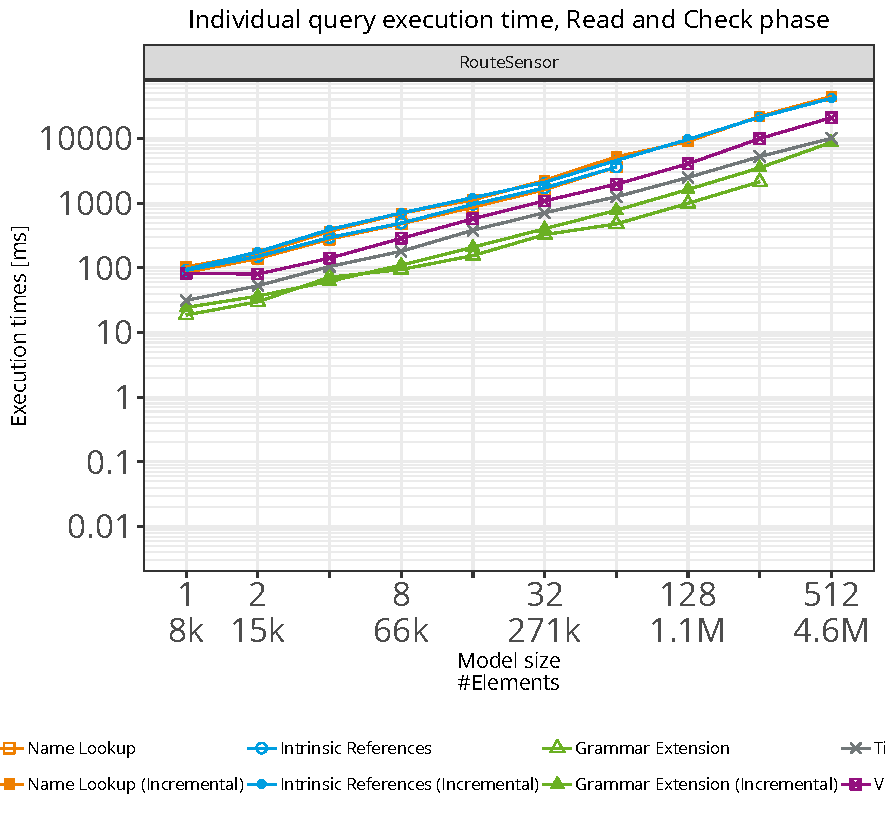
\includegraphics[height=10.5cm,keepaspectratio,clip,trim=0cm 4.2cm 0cm 1.35cm]{images/repair-Read-and-Check-RouteSensor.pdf}
\\[4mm]
\noindent\rotatebox{90}{\textbf{\hspace{28mm} Connected Segments}}
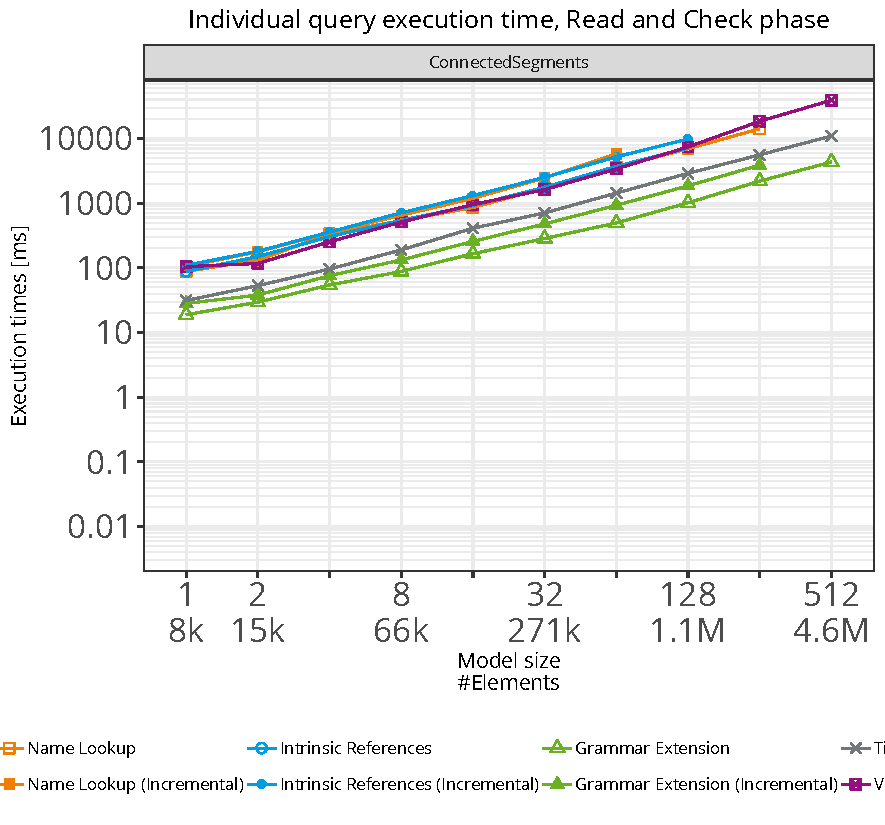
\includegraphics[height=13cm,keepaspectratio,clip,trim=0cm 2.2cm 0cm 1.35cm]{images/repair-Read-and-Check-ConnectedSegments.pdf}
\end{minipage}
%% Transformation and Recheck - Inject
\begin{minipage}{150mm}
\hspace{2mm} \textbf{Inject, Transformation + Recheck}\par\vspace{2mm}
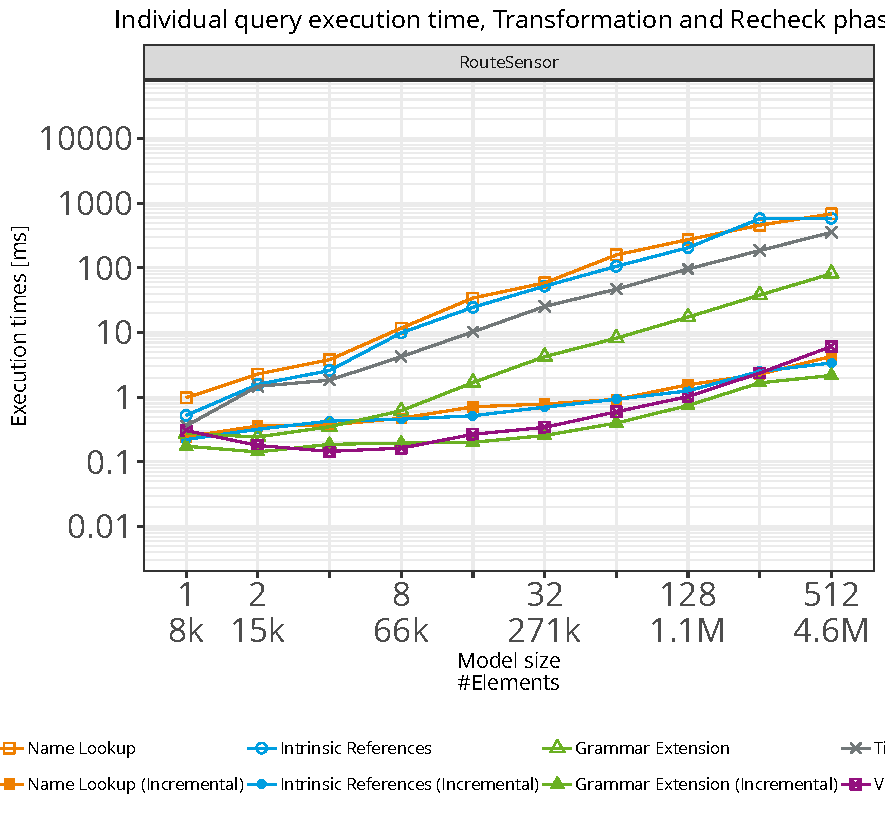
\includegraphics[height=10.5cm,keepaspectratio,clip,trim=2.3cm 4.2cm 0cm 1.35cm]{images/inject-Transformation-and-Recheck-RouteSensor.pdf}
\\[4mm]
\noindent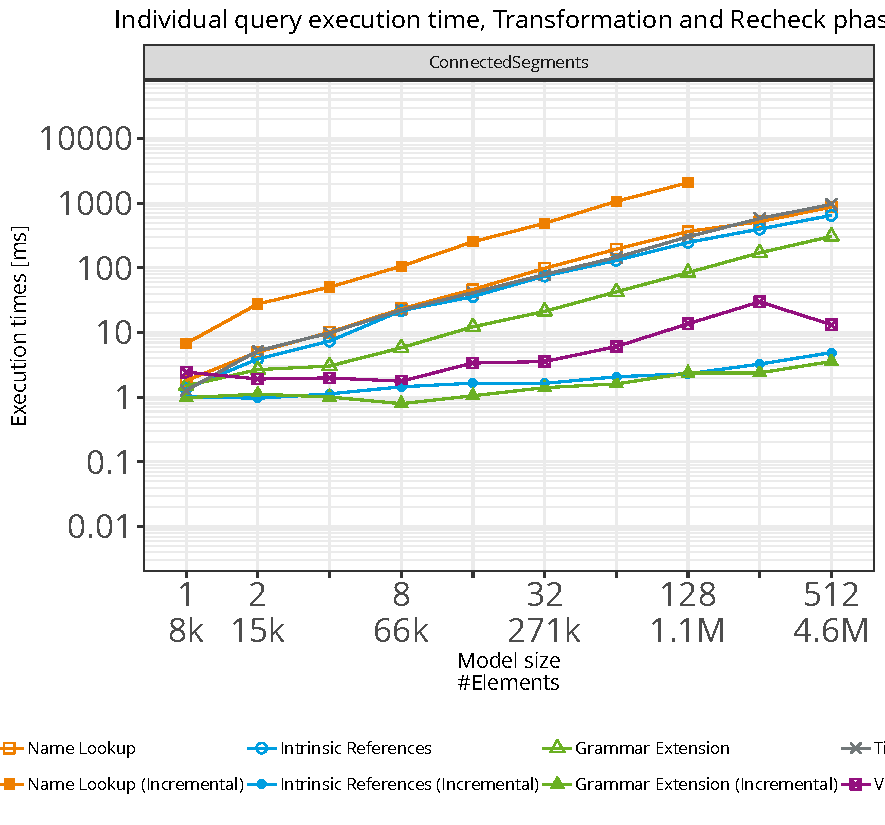
\includegraphics[height=13cm,keepaspectratio,clip,trim=2.3cm 2.2cm 0cm 1.35cm]{images/inject-Transformation-and-Recheck-ConnectedSegments.pdf}
\end{minipage}
%% Transformation and Recheck - Repair
\begin{minipage}{170mm}
\hspace{2mm} \textbf{Repair, Transformation + Recheck}\par\vspace{2mm}
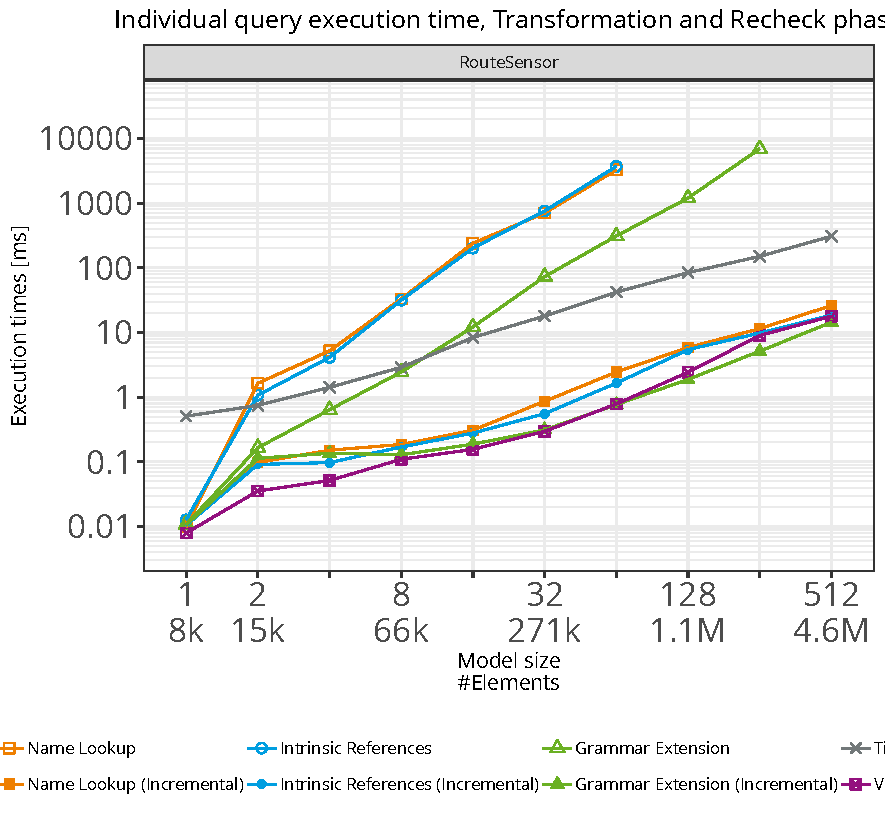
\includegraphics[height=10.5cm,keepaspectratio,clip,trim=2.3cm 4.2cm 0cm 1.35cm]{images/repair-Transformation-and-Recheck-RouteSensor.pdf}
\\[4mm]
\noindent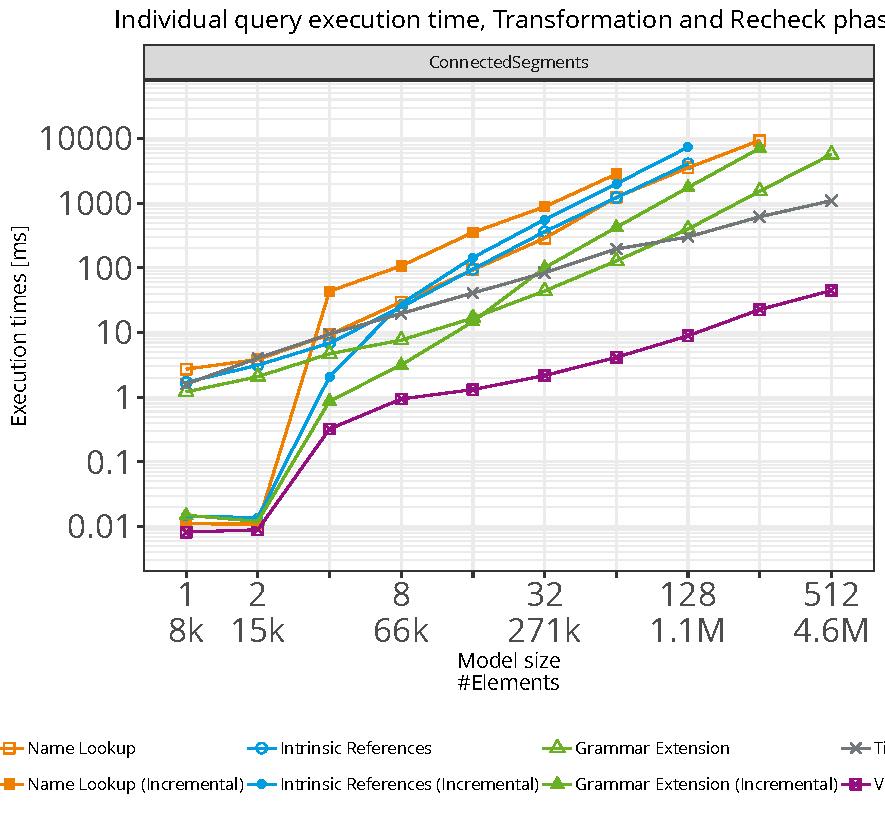
\includegraphics[height=13cm,keepaspectratio,clip,trim=2.3cm 2.2cm 0cm 1.35cm]{images/repair-Transformation-and-Recheck-ConnectedSegments.pdf}
\end{minipage}
%% Legend
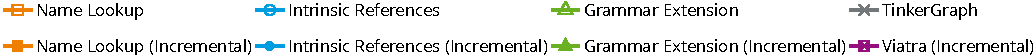
\includegraphics[width=530mm]{images/diagram-legend}
\end{minipage}
\clinesep%
\end{contentbox}
\titlebox{Continuous Model Validation using Reference Attribute Grammars}{Johannes~Mey\textsuperscript{1}, René~Schöne\textsuperscript{1}, Görel~Hedin\textsuperscript{2}, Emma~Söderberg\textsuperscript{2}, Thomas~Kühn\textsuperscript{1}, Niklas~Fors\textsuperscript{2}, Jesper~Öqvist\textsuperscript{2}, and Uwe~Aßmann\textsuperscript{1}\\[5mm]\small\textsuperscript{1}Technische Universität Dresden\\[-4mm]\textsuperscript{2}Lund University}
\begin{literaturebox}
\begingroup
\renewcommand{\section}[2]{}%
\bibliographystyle{plain}
\bibliography{references}
\endgroup
\end{literaturebox}

\begin{tikzpicture}[remember picture,overlay,
helpbox/.style={draw=red,anchor=north west},
helpline/.style={draw=red},
bluebox/.style={fill=HKS41,anchor=south west},
infobox/.style={fill=HKS44!15,anchor=north west},
]
\node at (current page.north west) {
	\begin{tikzpicture}[remember picture,overlay]
	\node[bluebox,minimum width=400mm,minimum height=84mm] at (32mm,-1169mm) {};
	\node[anchor=north west,color=white,font=\footnotesize] at (28mm,-1078mm) {
	\begin{minipage}{774mm}
	\textbf{Acknowledgments:} This work is partly supported by the German Research Foundation (DFG) in the SFB 912 “Highly Adaptive Energy-Efficient Computing”, the project “RISCOS” and within the Research Training Group “Role-based Software Infrastructures for continuous-context-sensitive Systems” (GRK 1907), and by the German Federal Ministry of Education and Research within the project “OpenLicht”. This work is also partly supported by the Swedish Governmental Agency for	Innovation Systems (VINNOVA) in the PIIA project 2017-02371 and by the Wallenberg AI, Autonomous Systems and Software Program (WASP) funded by the Knut and Alice Wallenberg Foundation (KAW).

	\end{minipage}
	};
	\node[text=white,anchor=north west,align=left] at (28mm,-1117.5mm) {
  \footnotesize\begin{tabular}{r@{\hskip 10mm}l@{\hskip 10mm}l@{\hskip 30mm}l@{\hskip 10mm}l}
		\textbf{Contact: } & Johannes Mey & \url{johannes.mey@tu-dresden.de} & Görel Hedin & gorel.hedin@cs.lth.se \\
    & René Schöne & \url{rene.schoene@tu-dresden.de} & Emma Söderberg & \url{emma.soderberg@cs.lth.se} \\
    & Thomas Kühn & \url{thomas.kuehn3@tu-dresden.de} & Niklas Fors & \url{niklas.fors@cs.lth.se}  \\
    & Uwe Aßmann  & \url{uwe.assmann@tu-dresden.de} & Jesper Öqvist & \url{jesper.oqvist@cs.lth.se} 
  \end{tabular}
%    \\[-6mm]
%		\scriptsize{Funding:}\\[-6mm]
%		\scriptsize{Spokesman:}\\[-6mm]
%		\scriptsize{Project Website:}
		};
%	\node[text=white,anchor=north west,align=left] at (87mm,-1147.5mm) {
%		\phantom{\scriptsize\textbf{Contact}} \\[-6mm]
%		\scriptsize{DFG (GRK 1907)}\\[-6mm]
%		\scriptsize{Prof. Dr.-Ing. Wolfgang Lehner}\\[-6mm]
%		\scriptsize{rosi-project.org}
%		};
	\end{tikzpicture}
};
\end{tikzpicture}


%\graduated
\end{document}
